\documentclass[11pt]{article}
\usepackage{graphicx}
\usepackage{enumitem}

%%%%%%%%%%%%%%%%%%%%%%%%%%%%%%%%%%%%%%%%%%%%%%%%%%%%%%%%%%%%%%%%%%%%%%%%%%%%%%%%
% packages
%%%%%%%%%%%%%%%%%%%%%%%%%%%%%%%%%%%%%%%%%%%%%%%%%%%%%%%%%%%%%%%%%%%%%%%%%%%%%%%%

\usepackage{coling2020}
\usepackage{times}
\usepackage{url}
\usepackage{amsmath,amsfonts}
\usepackage{latexsym}
\usepackage{hyperref}
\hypersetup{
  colorlinks   = true, %Colours links instead of ugly boxes
  urlcolor     = blue, %Colour for external hyperlinks
  linkcolor    = blue, %Colour of internal links
  citecolor    = blue  %Colour of citations
}
\usepackage{CJKutf8}
\usepackage[sort&compress,round,comma,authoryear]{natbib}

%%%%%%%%%%%%%%%%%%%%%%%%%%%%%%%%%%%%%%%%%%%%%%%%%%%%%%%%%%%%%%%%%%%%%%%%%%%%%%%%
% latex functions
%%%%%%%%%%%%%%%%%%%%%%%%%%%%%%%%%%%%%%%%%%%%%%%%%%%%%%%%%%%%%%%%%%%%%%%%%%%%%%%%

\newcommand{\ltwo}[1]{\lVert{#1}\rVert}
\newcommand{\indicator}[1]{\mathbbm{1}\!\left[{#1}\right]}
\newcommand{\R}{\mathbb R}
\newcommand{\TEXT}{\texttt{text}}

\newcommand{\defn}[1]{\emph{{#1}}}
\newcommand{\fixme}[1]{\textbf{FIXME: {#1}}}
\newcommand{\XXX}{\textbf{XXX}~}

\DeclareMathOperator*{\argmax}{arg\,max}
\DeclareMathOperator*{\argmin}{arg\,min}
\DeclareMathOperator{\acc}{acc}
\DeclareMathOperator{\none}{\texttt{None}}
\DeclareMathOperator{\model}{\texttt{BERTMultilingualEmoticon}}
\DeclareMathOperator{\emoticon}{\texttt{TwitterEmoticon}}
\DeclareMathOperator{\emoticonTrain}{\texttt{TwitterEmoticon\_train}}
\DeclareMathOperator{\emoticonValid}{\texttt{TwitterEmoticon\_valid}}
\DeclareMathOperator{\emoticonTest}{\texttt{TwitterEmoticon\_test}}
\DeclareMathOperator{\corona}{\texttt{TwitterCorona}}

%%%%%%%%%%%%%%%%%%%%%%%%%%%%%%%%%%%%%%%%%%%%%%%%%%%%%%%%%%%%%%%%%%%%%%%%%%%%%%%%
% paper configuration
%%%%%%%%%%%%%%%%%%%%%%%%%%%%%%%%%%%%%%%%%%%%%%%%%%%%%%%%%%%%%%%%%%%%%%%%%%%%%%%%

%\setlength\titlebox{5cm}
%\colingfinalcopy % Uncomment this line for the final submission

% You can expand the titlebox if you need extra space
% to show all the authors. Please do not make the titlebox
% smaller than 5cm (the original size); we will check this
% in the camera-ready version and ask you to change it back.


\title{Instructions for COLING-2020 Proceedings}

\author{First Author \\
  Affiliation / Address line 1 \\
  Affiliation / Address line 2 \\
  Affiliation / Address line 3 \\
  {\tt email@domain} \\\And
  Second Author \\
  Affiliation / Address line 1 \\
  Affiliation / Address line 2 \\
  Affiliation / Address line 3 \\
  {\tt email@domain} \\}

\date{}

%%%%%%%%%%%%%%%%%%%%%%%%%%%%%%%%%%%%%%%%%%%%%%%%%%%%%%%%%%%%%%%%%%%%%%%%%%%%%%%%
% document text
%%%%%%%%%%%%%%%%%%%%%%%%%%%%%%%%%%%%%%%%%%%%%%%%%%%%%%%%%%%%%%%%%%%%%%%%%%%%%%%%

\begin{document}
\maketitle
\begin{abstract}
\end{abstract}

%
% The following footnote without marker is needed for the camera-ready
% version of the paper.
% Comment out the instructions (first text) and uncomment the 8 lines
% under "final paper" for your variant of English.
% 
\blfootnote{
    %
    % for review submission
    %
    \hspace{-0.65cm}  % space normally used by the marker
    Place licence statement here for the camera-ready version. 
    %
    % % final paper: en-uk version 
    %
    % \hspace{-0.65cm}  % space normally used by the marker
    % This work is licensed under a Creative Commons 
    % Attribution 4.0 International Licence.
    % Licence details:
    % \url{http://creativecommons.org/licenses/by/4.0/}.
    % 
    % % final paper: en-us version 
    %
    % \hspace{-0.65cm}  % space normally used by the marker
    % This work is licensed under a Creative Commons 
    % Attribution 4.0 International License.
    % License details:
    % \url{http://creativecommons.org/licenses/by/4.0/}.
}

\section{Introduction}
\label{sec:intro}

\subsection{Contributions}

\begin{enumerate}
    \item 
        We introduce the $\emoticon$ dataset for training emotion prediction models.
    \item
        We introduce the $\model$ model for emotion prediction that fine tunes the \texttt{BERTMultilingual} model \citep{fixme} to the emotion prediction task. 
        $\model$ is the first multilingual model for emotion prediction,
        and we provide an open source Python interface wrapped in an easy to use PyPi package.
    \item
        We analyze the performance of our model with respect to different languages and cultures to provide the first cross-cultural analysis of emotion prediction.
    \item 
        We introduce the $\corona$ dataset of all geotagged tweets about the coronavirus sent before July 2020.
        We apply our $\model$ model to this dataset,
        and map out the public's emotional response to the coronavirus.
\end{enumerate}

\section{The Data}
\label{sec:data}

This section describes our two new Twitter datasets, $\corona$ and $\emoticon$.
To generate both datasets,
we first downloaded all geolocated\footnote{%
Twitter users can adjust their privacy settings to include different amounts of geolocation metadata.
In particular, they can include the exact GPS coordinate that a tweet was sent from,
an approximate location (for example, the city that the tweet was sent from),
or no location information at all.
We say that a tweet is \defn{geolocated} if any of this metadata is included about the tweet.
Approximate 1\% of all tweets are geolocated.
} 
tweets sent over the six month period from January 1st to June 30th, 2020.
This full dataset contains \XXX million tweets sent from \XXX users and from \XXX different countries.
The $\corona$ and $\emoticon$ datasets were then constructed by filtering this full dataset in different ways.

\subsection {The $\corona$ dataset}

The goal of the $\corona$ dataset is to include any geolocated tweet that references the coronavirus in any language.
We use a relatively complicated process to extract these tweets in order to ensure maximum recall and precision in a wide range of languages.
Our procedure is:
\begin{enumerate}
\item
We generated a list of \XXX English-language search terms related to the coronavirus,
such as \texttt{coronavirus}, \texttt{covid19}, \texttt{wuhan} and \texttt{lockdown}.
We then used Bing's translation API to translate each of these terms into the 72 languages supported by Bing translate.
Table \ref{table:search_terms} in the supplemental material contains the full list of search terms in English and selected translations.
\item
We used Python's \texttt{spacy} library \citep{fixme} to tokenize and lemmatize each of the \XXX million tweets in the full dataset.
\texttt{spacy} supports this process in 58 different languages,
and for each tweet we used the appropriate \texttt{spacy} module for the language specified in the tweet's metadata.
\item
Finally, the $\corona$ dataset is constructed as the set of all tweets whose lemmatized text contains any of the search terms from the tweet's language or English.
We include both languages in this filtering step because it is common for non-English tweets to use English words like \texttt{coronavirus} when referencing the virus.
\end{enumerate}
Table \ref{table:lang} shows the 54 languages that are supported by all 3 services along with the total number of tweets in each language.
Figure \ref{fig:corona:perday} provides a summary of the number of tweets per day and Figure \ref{fig:corona:spatial} shows the spatial distribution of the tweets.

\begin{table}
    \centering
    \includegraphics[height=2in]{example-image-a}
    \caption{The number of tweets in each language.} 
    \label{table:lang}
\end{table}

\begin{figure}
    \centering
    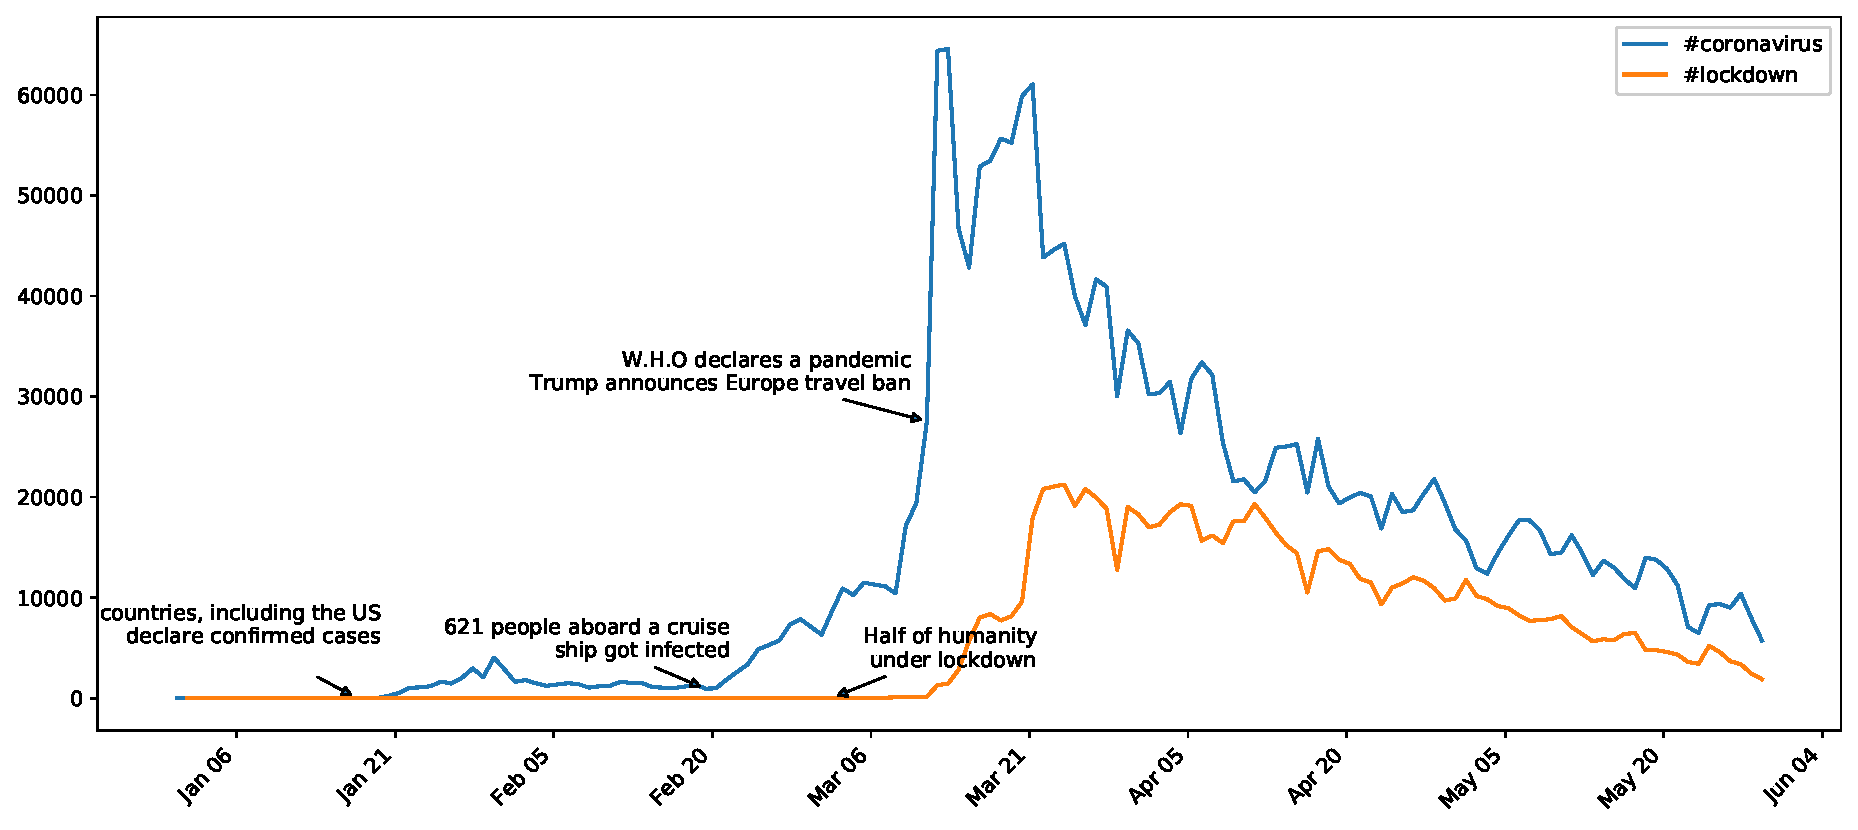
\includegraphics[width=\textwidth]{images/finalcountgraph1.eps}
    \caption{Number of tweets per day...}
    \label{fig:tweets_per_day}
\end{figure}

\begin{figure}
    \centering
    \includegraphics[height=2in]{example-image-a}
    \caption{The spatial distribution of the dataset.}
    \label{fig:corona:spatial}
\end{figure}

The other significant dataset of coronavirus related tweets is due to \citet{chen2020tracking}.
There are two main differences between our dataset and theirs.
First, we only include geolocated tweets,
whereas they include non-geolocated tweets as well.
This results in their dataset being about 50x larger than ours,
with about 250 million tweets over the same time period.
Because their data is not geolocated, however, their data is not suitable for the cultural analysis we perform in Section \ref{sec:}.
The second difference is that our dataset uses a more advanced language-aware filtering method.
They only search for tweets that contain English keywords.
Most languages, however, have few words in common with English,
and non-Latin based languages frequently do not even use the word \texttt{coronavirus} to describe the virus.
Chinese tweets, for example, commonly refer to the coronavirus with the string
\begin{CJK}{UTF8}{gbsn}
病毒
\end{CJK},
and Chinese-language tweets containing this string will get included in our dataset but not in their dataset.
As a result of this more advanced processing, the fraction of non-English tweets is much larger in our dataset than theirs (\XXX versus 38\%).
Again, this improves our multicultural analysis in Section \ref{sec:}.

We used NVidia's \texttt{sentiment-discovery} library to provide a preliminary sentiment analysis of the $\corona$ dataset,
and the results are shown in Figure \ref{fig:nvidia-sentiment}.
The results are not very informative, however, because NVidia's model was trained on a small set of English-language tweets (about 16 thousand) about video games,
and there is little reason to believe that this domain would transfer well to the coronavirus domain.

\begin{figure}
    %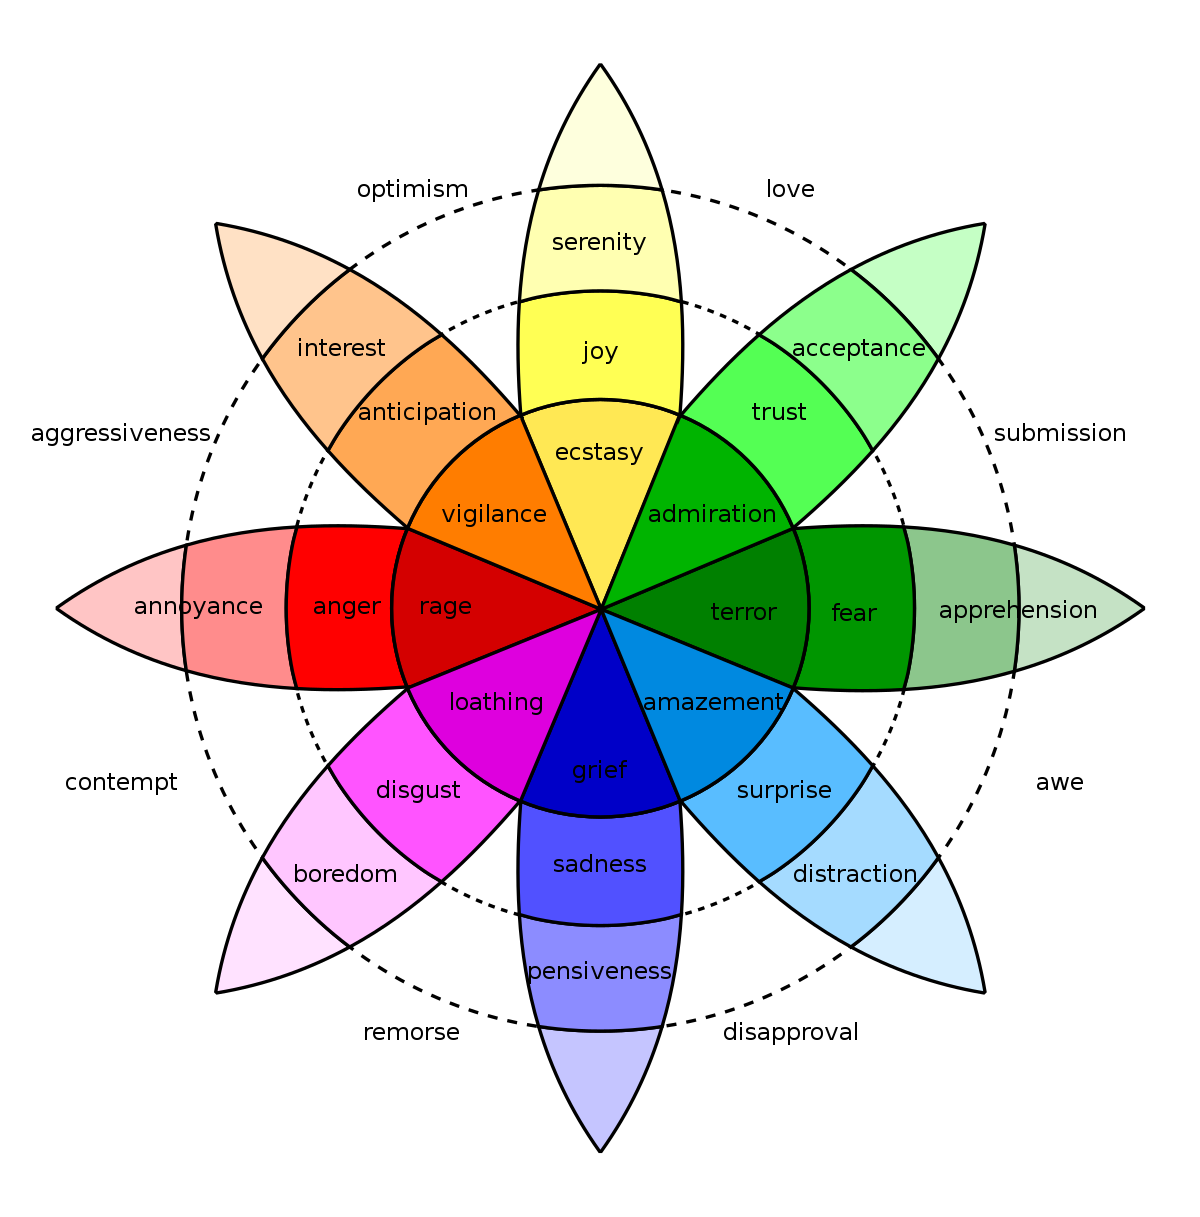
\includegraphics[width=0.4\textwidth]{images/Plutchik-wheel.png}
    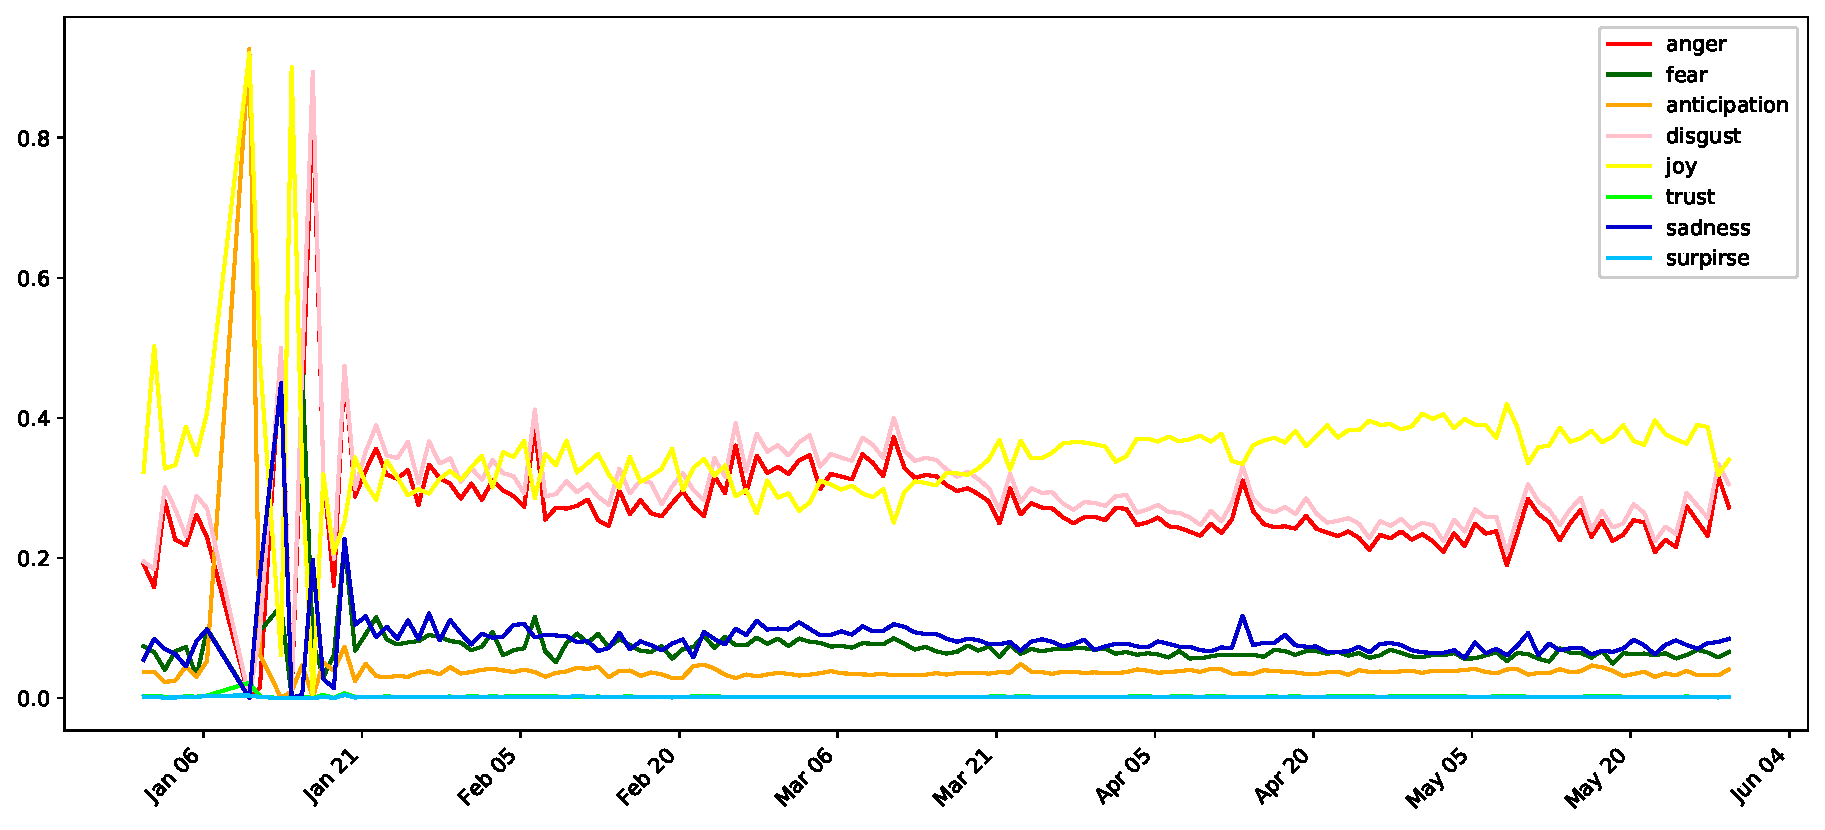
\includegraphics[width=\textwidth]{images/emotions.eps}
    \caption{Results of sentiment analysis conducted using nvidia-sentiment on 170k tweets related with the corona outrbreak }
    \label{fig:nvidia-sentiment}
\end{figure}

\subsection {The $\emoticon$ dataset}

The purpose of the $\emoticon$ dataset is to develop the emotion classifier which we will apply to the $\corona$ dataset.
The $\emoticon$ dataset is large, with \XXX million tweets in 66 languages sampled from the same distribution as our coronavirus tweets.
Therefore, we can expect a classifier trained on the $\emoticon$ dataset to transfer well to the $\corona$ dataset.

Following the work of \citet{fixme1,fixme2,fixme3}, we use emojis as distant labels for emotions.
Hand classifying text by emotions is an expensive and error prone process,
and the largest existing datasets for this task contain only about 10,000 tweets focusing on the limited domains of video games \citep{fixme} or stock performance \citep{fixme}.
The Unicode Standard \citep{fixme} currently defines over 3000 emojis,
most of which do not represent emotions.
In our analysis, we use only the original 80 emoji defined in the Unicode standard's emoticon code block (code points \texttt{0x1f600} - \texttt{0x1f650}).\footnote{
    In common usage, the words \defn{emoji} and \defn{emoticon} are interchangeable,
    but in this paper we adopt the Unicode Standard's definitions of these terms.
    By these definitions, an \defn{emoji} is any one of 3304 pictographs that are not part of any written language,
    and an \defn{emoticon} is one of the original 80 emoji.
}
We limit are analysis to emoticons only because:
they are the most commonly used emoji on twitter\footnote{
    See \url{http://www.emojitracker.com/} for realtime stats on Twitter emoji usage.
}
and each of these emoticons represents an emotion (emoticon is a portmanteau of emotion and icon).

To generate the $\emoticon$ dataset, 
we filtered the full set of geolocated tweets so that only tweets containing one of the 80 emoticons were included,
and any duplicate tweets were removed.
Then we preprocessed each tweet by replacing all user mentions with a special token \texttt{<mention>} and all URLs with a special token \texttt{<url>} and deleting all emojis.
We decided to keep all hashtags because hashtags can contain potentially valuable emotional content.
Finally, each tweet is labelled with the emojis that were deleted from the tweet.

In total, the $\emoticon$ dataset contains 64.2 million tweets sent by 4.2 million users,
and the tweets are written in 66 different languages and were sent from 246 different countries.
Table \ref{table:lang} shows the total number of tweets per language,
and Figure \ref{fig:emoticons} shows the full list of emoticons and their counts in our dataset. 

\begin{figure}
    \centering
    \includegraphics[height=2in]{example-image-a}
    \caption{Emoticons image.}
    \label{fig:emoticons}
\end{figure}

Our goal with this dataset is to construct a classifier that takes as input a tweet and outputs an emoticon that represents the emotion of the tweet.
In order to train this model properly,
we carefully split the $\emoticon$ dataset into training, validation, and test sets ensuring that no user is present in all three sets in order to prevent data leakage.
In particular we assign 80\% of users to the training set, 10\% to the validation set, and 10\% to the test set.
The tweets contained in each set are then the tweets sent by each of the users in the set.

Importantly, duplicate tweets are included in the $\corona$ dataset,
but they are not included in the $\emoticon$ dataset.
\fixme{Can you come up with an explanation about why this is good or bad?}

\section{Experiments}
\label{sec:experiments}

We now describe how we trained our $\model$ model on the $\emoticon$ dataset.
Then we apply this model to the $\corona$ dataset to label millions of previously unlabelled tweets about the coronavirus with emotions.
We use these emotion labels to then show how different people around the world have reacted to the coronavirus.

\subsection{Training procedure and performance on $\emoticon$}

\subsection{Performance on $\corona$}


\section{Related Work}
\label{sec:related}
\subsection{Stefanos}
Datasets: 

DENS: A Dataset for Multi-class Emotion Analysis:By finetuning the pre-trained uncased BERT-large to a multi-class passage classification task they achieved a micro-F1 score of 60.4\%. 



%\cite{liu2019dens}

%\cite{SemEval2018Task1}

Pretrained models:

%\cite{puri2018large}

%\cite{kant2018practical}

Examples of large scale sentiment analysis:

%\cite{mohammad2015sentiment}

%\cite{hemmatian2017survey}

%\cite{yang2015twitter}


\section{Discussion}
\label{sec:discussion}


%\bibliographystyle{coling}
\bibliographystyle{plainnat}
\bibliography{main}

\end{document}
